\section{V14}
\subsection{Prinzip der Genotyp-Imputation}
\textbf{Hintergrund:} bei nichteindeutiger Clusterzuordnung der Intensitäten beider Allele wird Genotyp auf „fehlend“ gesetzt $\rightarrow$ „Löcher“ im Datensatz\\\\
$\rightarrow$ durch Imputation können diese fehlenden Genotypen geschätzt und ersetzt werden\\\\
\textbf{Mögliches Vorgehen:}
\begin{itemize}
	\item Ausfüllen der Löcher im Datensatz ohne Referenz
	\item Ausfüllen der Löcher im Datensatz mit Referenz
	\item Schätzen von nichtgemessenen Genotypen mittels Referenz
\end{itemize}

\textbf{Nutzen:}
\begin{itemize}
	\item Vervollständigen der Daten für Analysezwecke
	\item Konstruktion einer gemeinsamen Marker-Menge für genetische Metaanalysen von Studien mit unterschiedlichen Genotypisierungsplattformen
	\item Erhöhung der Power
	\item Korrektur von Genotypisierungsfehlern (in geringem Maße)
\end{itemize}

\textbf{Problem:}
\begin{itemize}
	\item Imputation ist ein Schätzverfahren
	\item Unsicherheit der resultierenden Genotypen muss bei der nachfolgenden Analyse geeignet berücksichtigt werden
\end{itemize}

\subsection{Aufbau eines HMMs}
\textcolor{red}{siehe Vorlesung}

\newpage
\subsection{Probleme des Referenzabgleichs}
Problem: Die Daten müssen zur Referenz insbesondere deren Annotationen passen\\\\
Wichtige Informationen zu SNP-Daten werden mit zwei Versionsangaben versehen:
\begin{itemize}
	\item \textbf{NCBI build (reference genome)}
	\begin{itemize}
		\item Angaben zur Lage der SNPs im humanem Genom
		\item betrifft Chromosom und Basenposition
		\item beides kann sich zwischen Versionen verändern
	\end{itemize}
	\item \textbf{dbSNP build}
	\begin{itemize}
		\item Database of single nucleotide polymorphisms (SNPs) and	multiple small-scale variations
		\item gelistete SNPs werden auf Referenzgenom gemappt
		\item alle SNPs erhalten eine offizielle “rsID” als SNP identifier (ändert sich zwischen Versionen!)
	\end{itemize}
\end{itemize}

\textbf{Vorgang}
\begin{enumerate}
	\item Eigene SNPs brauchen eine rsID: Falls keine gefunden, muss SNP gefiltert werden oder über Position auf Referenz abgebildet werden
	\item NCBI build der eigenen Daten muss mit dem des
Referenzdatensatzes übereinstimmen: Falls nicht gegebenen, muss einer der Datensätze geliftet werden (vorzugsweise der eigene Datensatz)
	\begin{itemize}
		\item Hilfreiches Tool: LiftOver der UCSC (später)
		\item Liftet SNPs anhand der gegebenen Positionen von einer Version des Human Genomes (HG-Version) zur nächsten
		\item ändert nur Positionsangaben, die richtigen rsIDs für neue Positionen müssen selbst gesucht werden
		\item dabei können SNPs verloren gehen
	\end{itemize}
	\item dbSNP build Identifier der eigenen Daten muss mit dem des Referenzdatensatzes übereinstimmen: Falls nicht gegeben, muss über die Positionsangaben aus dem gewünschten dbSNP build die korrekte rsID ermittelt werden
	\begin{itemize}
		\item Achtung: für einige Positionen gibt es mehrere rsIDs
		\item wenn möglich, rsID des Referenzdatensatzes übernehmen
	\end{itemize}
	\item SNP-Informationen sollten zwischen Referenz und eigenem Datensatz übereinstimmen
	\begin{itemize}
		\item identische Positionsangaben
		\item identische rsIDs
		\item identische Basenkombination (bzgl. des richtigen Strangs)
		\item Letzteres erfordert erfahrungsgemäß die meisten Probleme insbesondere bei A/T, C/G SNPs und Frequenzen nahe 50\%
		\item Alle SNPs mit ungeklärten Widersprüchen sollten aus den eigenen Daten gefiltert werden, werden „mit etwas Glück“ durch Imputation wieder eingebracht
	\end{itemize}
\end{enumerate}

\subsection{Messen der Imputationsqualität}
Imputation liefert zwei relevante Wahrscheinlichkeiten:
\begin{itemize}
	\item $p_1$ = Wahrscheinlichkeit für Heterozygot
	\item $p_2$ = Wahrscheinlichkeit für Homozygot BB
\end{itemize}

Wenn die wahren Genotypen bekannt sind, kann man Maße der
Imputationsgüte über Abstände von Verteilungen definieren:
\textcolor{red}{Was ist das alles???}
\\\\
Die wahren Genotypen sind i.d.R. jedoch nicht bekannt. Die Imputations-
güte wird dann aus der Abweichung der geschätzten Genotypverteilung
von der zufällig erwarteten (durch Raten) ermittelt:\\
Alleldodid B des i-ten Individuums des j-ten SNPs: $e_{ij}=p_{ij1}+2p_{ij2}$\\
\textcolor{red}{???}: $f_{ij}=p_{ij1}+4p_{ij2}$\\
Empirische Allelfrequenz des j-ten SNPs: $\hat{\theta}=\frac{\sum_{i=1}^{N}e_{ij}}{2N}$
\\\\
\textbf{MaCH r$^2$}\\
empirische Varianz der Gendosen geteilt durch die unter HWE erwartete Varianz\\
$\hat{r}^2_j=
\begin{cases}
    \frac{\frac{\sum_{i=1}^{N}e^2_{ij}}{N} - (\frac{\sum_{i=1}^{N}e_{ij}}{N})^2}{2\hat{\theta}(1-\hat{\theta})}  & \quad \text{when } \hat{\theta} \in (0,1)\\
    1  & \quad \text{when } \hat{\theta}=0, \hat{\theta}=1\\
\end{cases}
$
\\\\
\textbf{IMPUTE info score}\\
1-Varianz der geschätzten Genotypen / Varianz der Genotypen bei zufälliger Stichprobenziehung mit $\theta$\\
$
I_A=
\begin{cases}
    1 - \frac{\sum_{i=1}^{N}(f_{ij}-e^2_{ij})}{2N\hat{\theta}(1-\hat{\theta})} & \quad \text{when } \hat{\theta} \in (0,1)\\
    1  & \quad \text{when } \hat{\theta}=0, \hat{\theta}=1\\
\end{cases}
$

führt zu Plot:\\
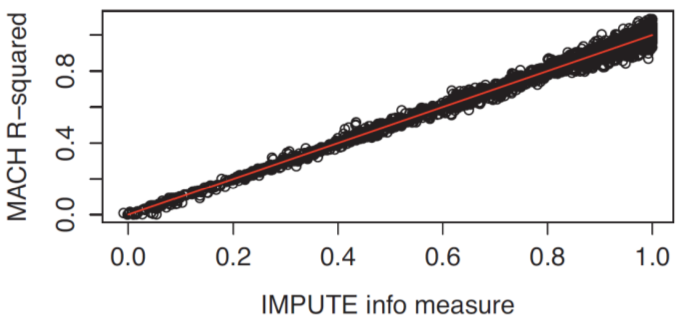
\includegraphics[width=1\textwidth]{lectures/V14/pix/machr_ia_plot.png}

\subsection{Einflußfaktoren auf die Imputationsqualität}
\begin{itemize}
	\item Referenzgenom
	\item Software (auf Ethnien)
\end{itemize}

\subsection{Problematik der Assoziationsanalyse mit imputierten Genotypen}
Die Unsicherheit bei der Imputation von Genotypen muß bei der Analyse berücksichtigt werden.\\

\underline{\textbf{Variante 1 (best-guess genotype):}} Man nimmt den Genotyp mit der höchsten posterior-Wahrscheinlichkeit und rechnet mit diesem weiter. Mitunter werden dabei zu geringe posterior-Wahrscheinlichkeiten auf „missing“ gesetzt (=neue Löcher).
\\\\
\underline{\textbf{Variante 2 (Alleldosis):}} Man bestimmt die Erwartung der posterior-Verteilung (=Alleldosis) und rechnet mit dieser weiter.
\\\\
\underline{\textbf{Variante 3 (Mischmodell):}} Man fittet ein Mischmodell an (nicht zu verwechseln mit „mixed model“!).
\\\\
z.B. Additives Modell:\\
$f_k(\mu,\beta,\epsilon_i)=
\begin{cases}
     \mu + \epsilon_i, & \quad k=0\\
     \mu + \beta + \epsilon_i, & \quad k=1\\
     \mu + 2\beta + \epsilon_i, & \quad k=2\\
\end{cases}
$\\

$y_i=\displaystyle \sum_{k=0}^2 p_{ki}f_k(\mu, \beta, \epsilon_i)$\\
Erfordert numerische Optimierung der Likelihood $\rightarrow$ Höherer Rechenaufwand
\\\\
\underline{\textbf{Variante 4 (Score-Test):}} Wird als „state of the art“ angesehen\\
Score-Funktion (L=Likelihood, $\theta$=genetischer Effekt): $U(\theta)=\frac{\delta log L(x,\theta)}{\delta \theta}$\\\\
Fisher-Information: $I(\theta)=-E[\frac{\delta^2}{\delta \theta^2} log L(x,\theta)]$\\\\
Verteilung unter H$_0$: $S(\theta_0)=\frac{U(\theta_0)^2}{I(\theta_0)} \sim \chi_1^2$
\\\\
Problematisch ist die mangelnde Stabilität dieses Ansatzes, bei kleinen Allelfrequenzen!